\documentclass[a4paper,10pt]{article}

\usepackage[utf8]{inputenc}
\usepackage[T1]{fontenc}
\usepackage[french]{babel}
\usepackage{float}
\usepackage{afterpage}
\usepackage[backend=bibtex]{biblatex}
\usepackage{graphicx}
\bibliography{definition}

\usepackage{hyperref}

\title{Régulation d'un système dynamique : application à une serre}
\author{A. Caccia \and A. Madeira Cortes \and N. Marchant \and R. Fontaine}
\date{ }

\begin{document}

\maketitle

\vspace{1cm}

\section{Sujet}

Le but du projet est de modéliser et gérer dynamiquement l'environnement d'une serre. Plusieurs variables seront mesurées et devront être maintenues dans des bornes acceptables pour les plantes: humidité du sol et de l'air, luminosité et température. Ces variables seront mesurées grâce des capteurs installés dans la serre. \\

Lorsque ces variables dépassent des bornes supérieure ou inférieure acceptables, le logiciel développé activera des dispositifs pour les rétablir entre ces bornes. C'est à dire: \\

\begin{enumerate}
	\item La température est régulée par une résistance chauffante et un ventilateur.
	\item L'humidité de l'air est régulée par un brumisateur et le ventilateur.
	\item L'humidité de du sol est régulée par un système d'irrigation.
	\item La luminosité est régulée par une lampe et un système de volets.\\
\end{enumerate}

\newpage

\section{Implémentation}

Le projet sera implémenté en plusieurs parties :

\begin{enumerate}
    \item La mesure des variables du système
    \item Le filtrage de ces mesures
    \item L'algorithme de contrôle en lui-même (probablement PID, voir \cite{Kinnaert2013})
    \item Exécution des commandes de correction (déterminées à l'étape précédents) par le matériel.
\end{enumerate}

La mesure de l'état du système sera fait à l'aide d'un Arduino et de capteurs analogiques simples à notre disposition à UrLab (le hackerspace de l'ULB). L'Arduino transmettra ensuite ces valeurs à un ordinateur qui filtrera ces données pour

MIMO Multiple Input Multiple Output \\

Algorithme PID, variantes, et autres algorithmes.\\

L'affichage des données sera pris en charge par un visualiseur dédié à l'affichage de données sous forme de graphes: Grafana. Il est possible d'afficher un historique avec des bornes délimitées (en bleu et rouge sur la figure suivante). \\

\thispagestyle{empty}
\begin{figure}[H]
\centering
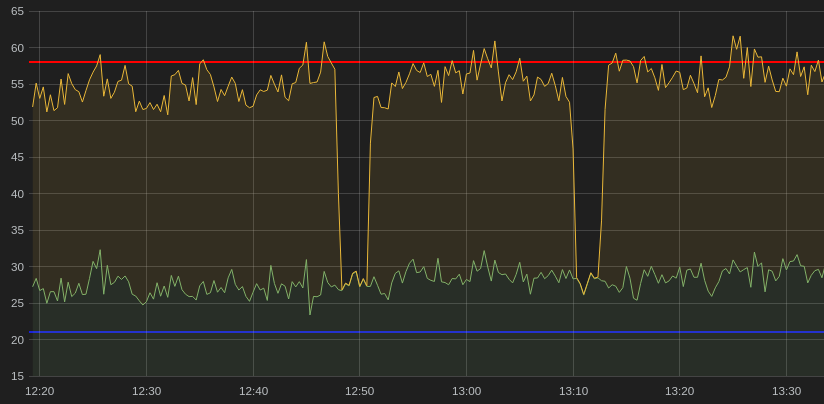
\includegraphics[scale=0.5]{figures/Grafana.png}
\caption{Grafana affichant des données}
\label{grafana}
\end{figure}

\section{Dispositif de présentation au Printemps des Sciences}

Lors du Printemps des Sciences, nous envisageons de présenter notre projet en exposant une serre où sont cultivées des fraises. \\

L'état des variables contrôlées dans la serre seraient affichées sur un écran, avec un historique visible et les bornes délimitées (comme détaillé dans la partie "Implémentation"). \\

Pour rendre la présentation dynamique et interactive, nous pourrions volontairement perturber le système et celui-ci se stabiliserait tout seul. Nous pourrions par exemple :
\begin{enumerate}
	\item Allumer une lampe et qu'en réaction le système ferme les volets.
	\item Chauffer la serre avec un dispositif externe (par exemple, un sèche-cheveux) pour que la ventilation s'enclenche.
	\item Autres... \\
\end{enumerate}

\section{Bibliographie}

Les deux premières sources sur lesquelles nous nous basons sont \citetitle{Kinnaert2013} \cite{Kinnaert2013} et \citetitle{Knospe2006} \cite{Knospe2006}, des cours détaillant les bases de l'algorithme PID. \\

Ensuite, nous ferrons référence à l'article \citetitle{Zheying2014} \cite{Zheying2014}. Il présente un cas d'étude très proche du notre en utilisant une version "fuzzy" de l'algorithme PID.\\

Deux documents présentent des implémentations concrètes proches de la notre: \citetitle{Ioannidis2014} \cite{Ioannidis2014} qui utilise un Raspberry Pi et \citetitle{ATMEL2005} \cite{ATMEL2005} qui utilise un microcontrôleur. \\

Pour présenter des variantes à l'algorithme PID, nous nous référerons à \citetitle{Afou2014} \cite{Afou2014}, \citetitle{ballard1993pid} \cite{ballard1993pid} et \citetitle{Saletovi2014} \cite{Saletovi2014} \\

Pour finir, nous envisageons d'utiliser des filtres de Kalman pour filtrer le signal en entrée du PID pour ne pas amplifier le bruit, et éventuellement prédire l'état futur du système. Nous nous basons sur l'article \citetitle{Welch2006} \cite{Welch2006}.

\newpage

\printbibliography

\end{document}
